% !TEX TS-program = XeLaTeX
% !TEX encoding = UTF-8 Unicode

\chapter{数据介绍与数据分析}
\label{chap01}

\section{数据集一特征提取与特征分析}
\subsection{数据集一的描述}
数据一为kaggle竞赛中一个连锁超市的数据,该比赛是通过各种特征来预测接下
来的销量,从而进行销售指导,平衡供求关系,减少额外的配送费用,其提供的原
始数据集有如下几个文件:
\begin{table}[htbp]  
  \centering
  \bicaption[tab:data1]{表}{数据一原始信息表}{Tab.}{data1}
  \vspace{0.2cm}
  \zhongwu
  \begin{tabularx}{0.8\textwidth{}}{lX}
    \toprule
    原始文件  				& 文件描述  \\
    \midrule
    train.csv 				& 训练数据,包含日期,店铺,售出的商品 \\
    stores.csv   			& 各个店铺的详细信息,比如商店的位置和商店的类型 \\
    items.csv   			& 商品的特征,比如是否易腐坏,商品类别等 \\
    transactions.csv    	& 训练数据中每个店铺的销售数额  \\ 
    oil.csv 				& 每日的原油价格  \\ 
    holidays\_events.csv 	& 假期信息  \\ 
    \bottomrule
  \end{tabularx}
\end{table}

其中train.csv文件中包括如下几列:id,date,store\_nbr,item\_nbr,
unit\_sales,onpromotion;分别表示日期,商店id,商品id,销量和是否正在
促销。对该文件的数据进行可视化,如图1.1所示,可以发现如下几点信息:
\begin{figure}[htbp]
  \centering
  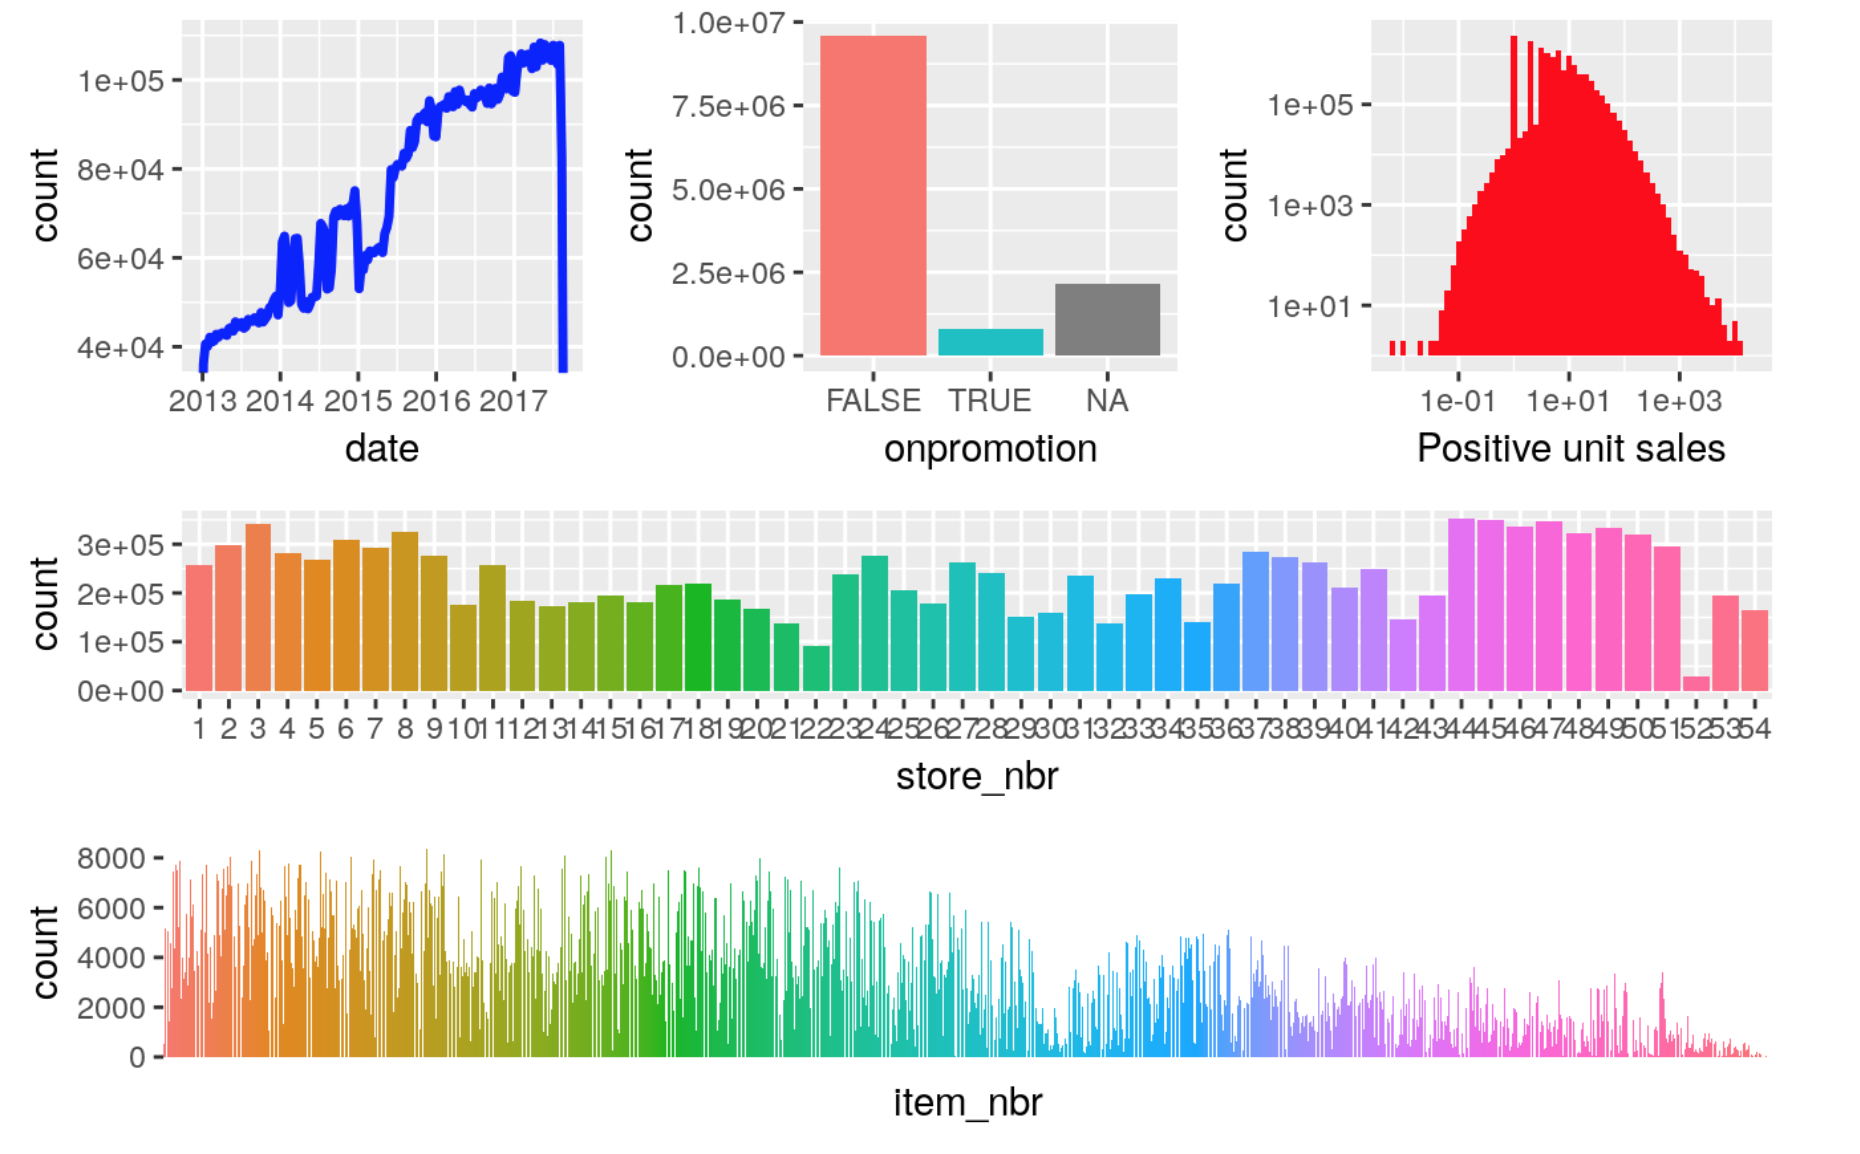
\includegraphics[width=\textwidth{},keepaspectratio]{traindescripe.png}
  \bicaption[fig:traindescripe]{图}{train.csv数据可视化图}{Tab.}{description of train.csv}
\end{figure}

\begin{asparaenum}
\item 随着时间的增加,销量整体呈现上升趋势。 
\item onpromotion是否在促销列有着大约五分之一的缺失值,且促销产品占比不大。
\item 数据中一共有着54个店铺和大量的商品。
\end{asparaenum}

其中stores.csv文件中包括如下几列:store\_nbr,city,state,type,cluster
分别代表着商店id,商店所在的城市,商店所在的州,商店的类型,其中,商店的类型
包括(A,B,C,D)四个类型,以及相似商店的聚类结果。对其进行可视化,可以发现
如下几点信息:
\begin{figure}[htbp]
  \centering
  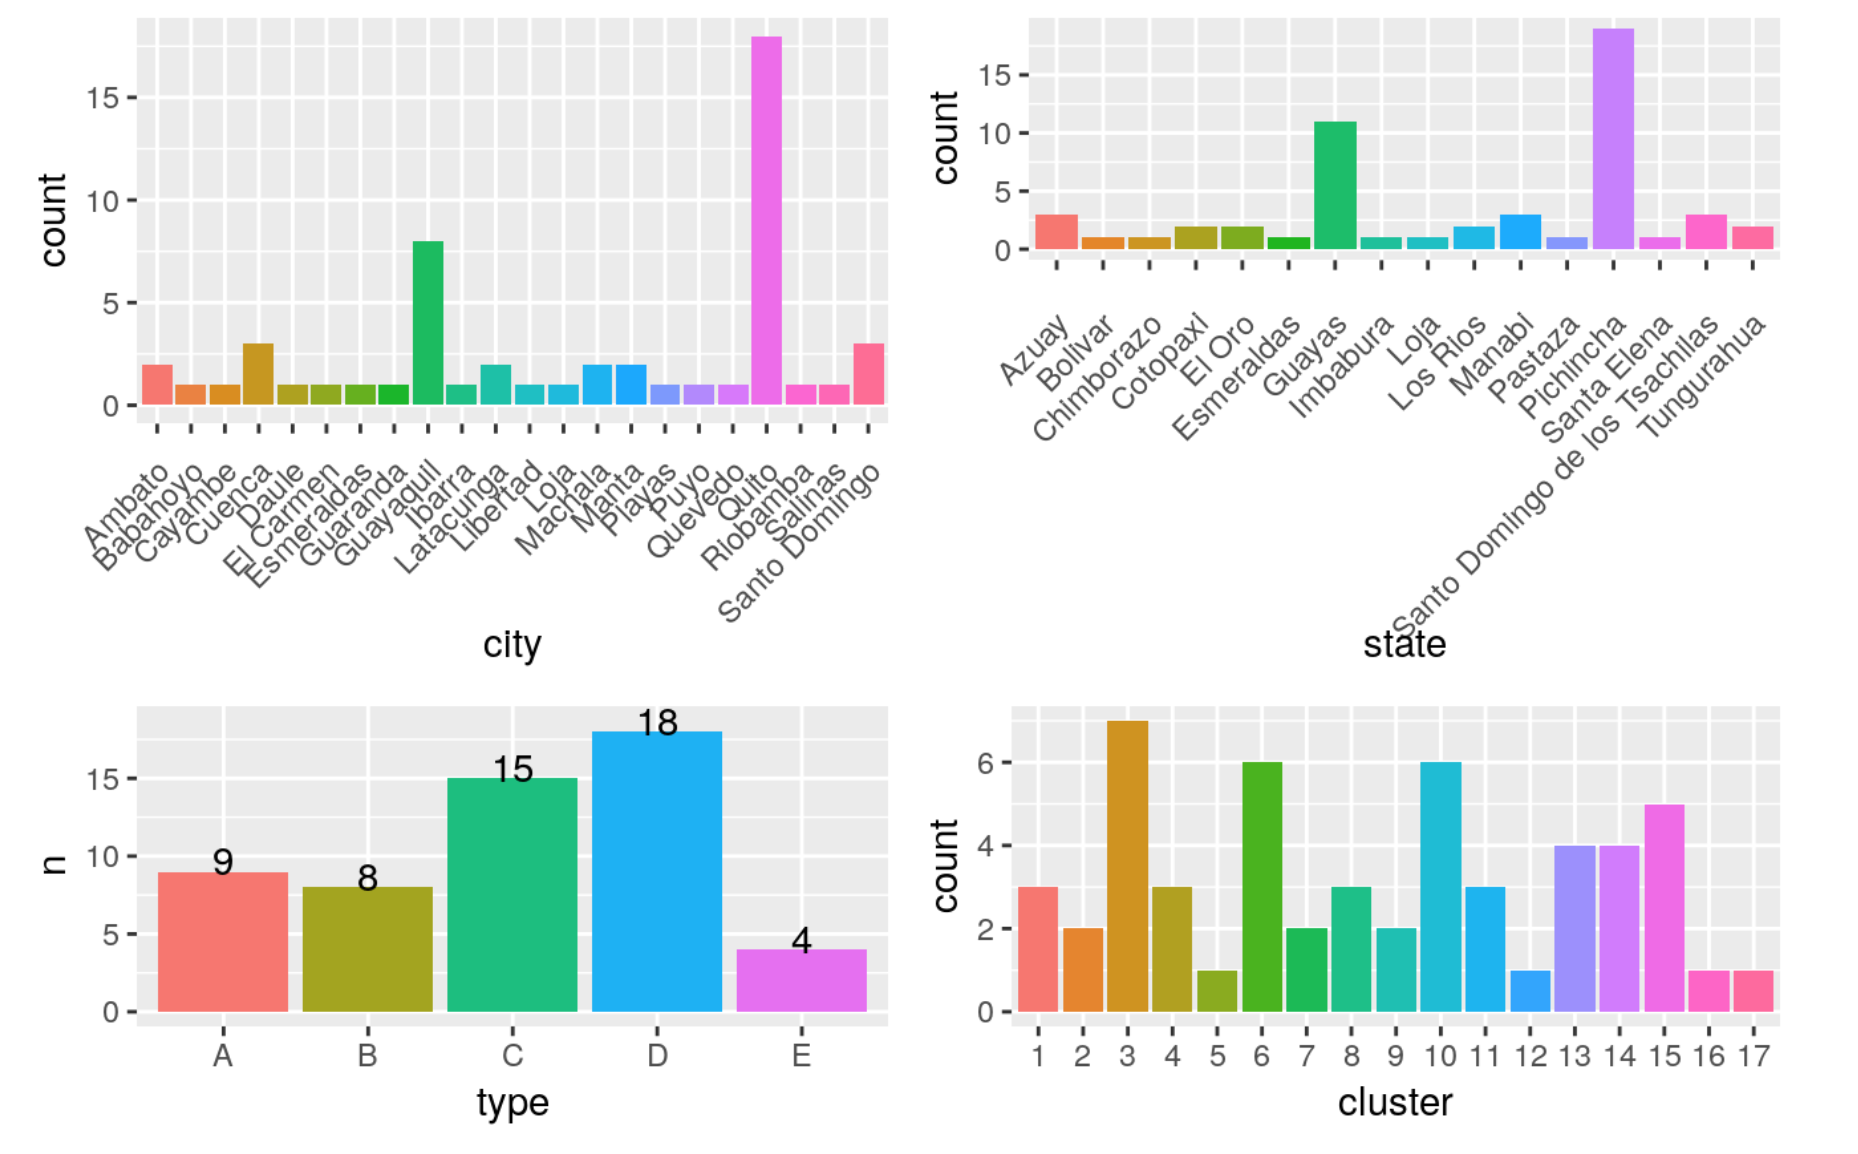
\includegraphics[width=\textwidth{},keepaspectratio]{storesdescripe.png}
  \bicaption[fig:storesdescripe]{图}{stores.csv数据可视化图}{Tab.}{description of stores.csv}
\end{figure}

\begin{asparaenum}
\item 各个商店分布在不同的州,市
\item C类型和D类型的店铺较多
\item 一共有17个不同的cluster
\end{asparaenum}


其中items.csv文件中包括如下几列:item\_nbr,family,class,perishable
分别代表着商品id,商品家族,商品的类别,易腐程度。
如下几点信息:
\begin{figure}[htbp]
  \centering
  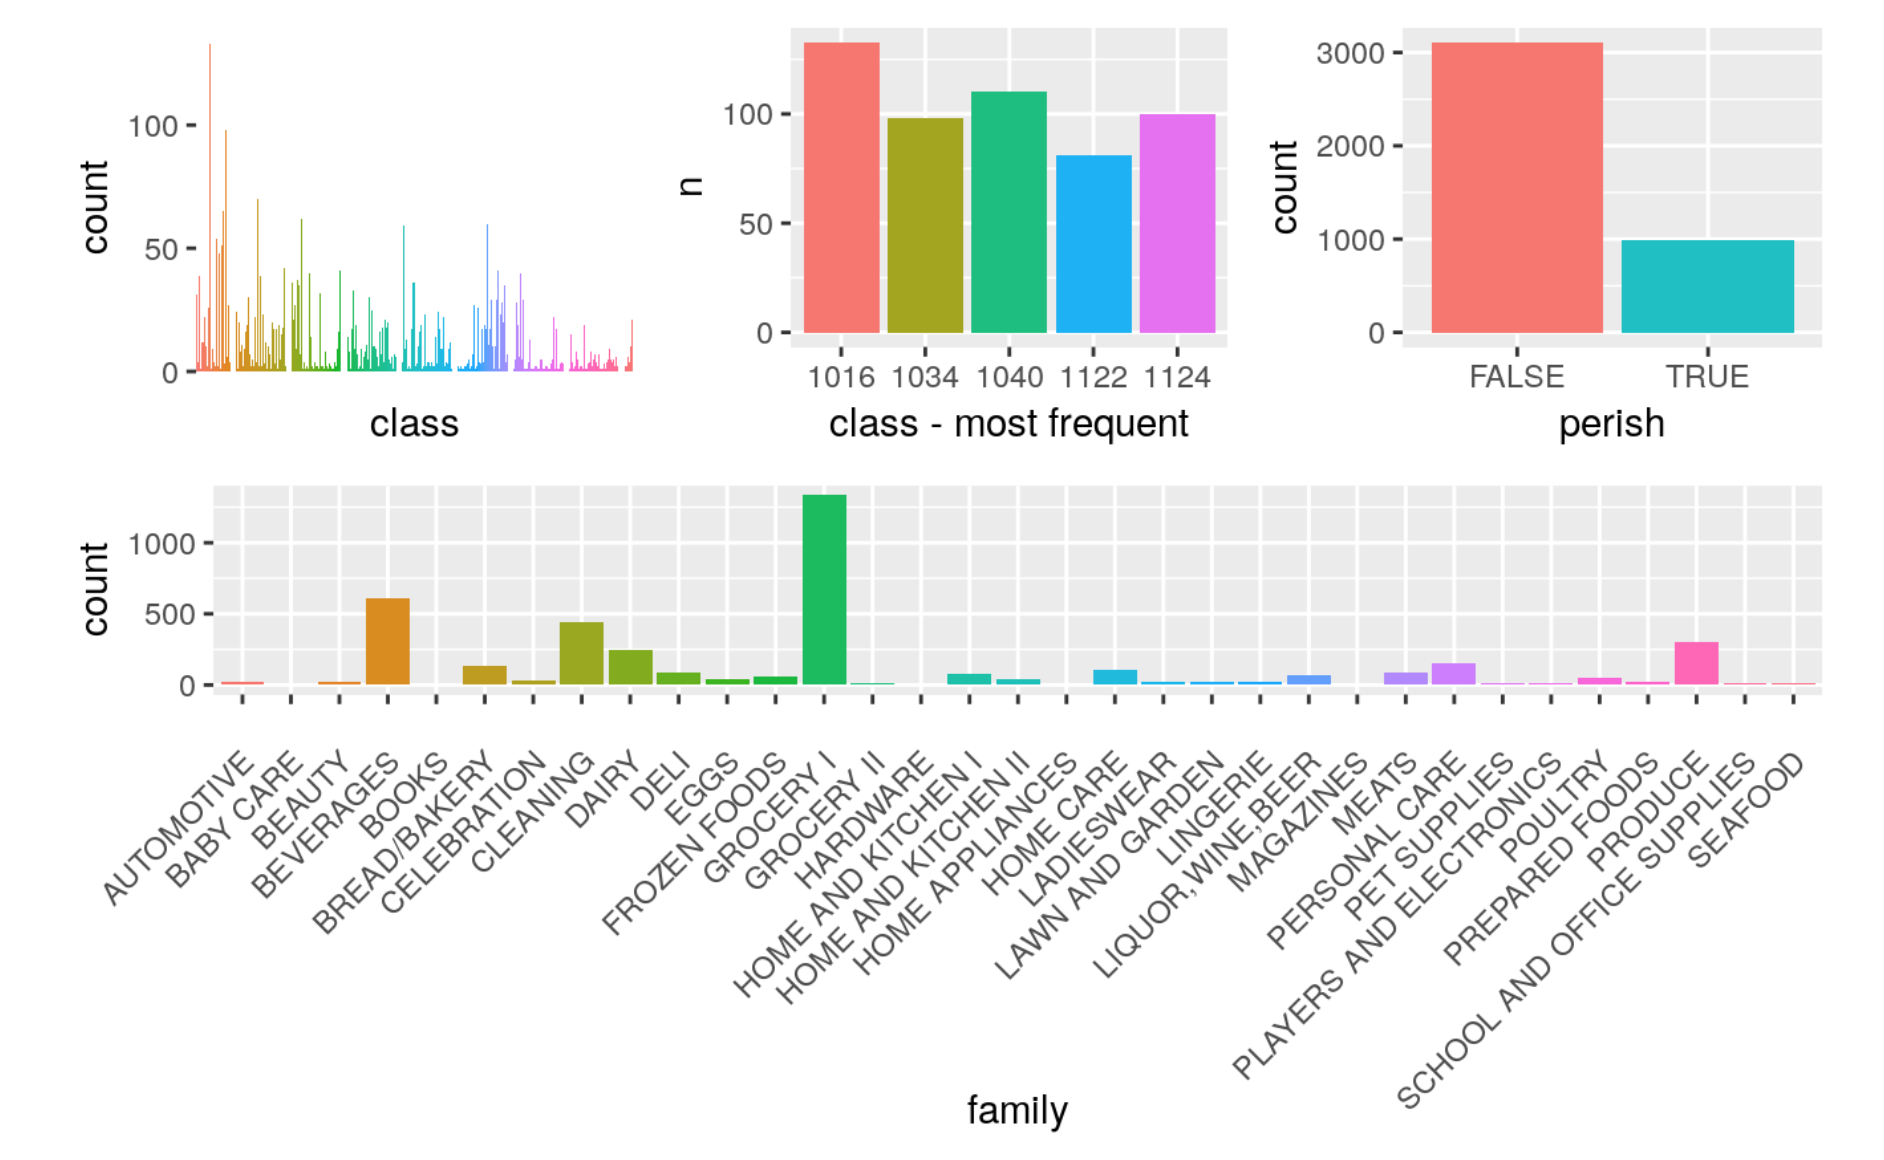
\includegraphics[width=\textwidth{},keepaspectratio]{itemsdescripe.png}
  \bicaption[fig:itemsdescripe]{图}{items.csv数据可视化图}{Tab.}{description of items.csv}
\end{figure}

\begin{asparaenum}
\item 各个商店分布在不同的州,市
\item C类型和D类型的店铺较多
\item 一共有17个不同的cluster
\end{asparaenum}






\section{数据集二特征提取与特征分析}
中英文摘要和关键字也位于~{/preface/cover.tex}~文件中,分别定义
在cabstract, eabstract, ckeywords, ekeywords中,替换成自己的即可。

这里附上研究生院对摘要和关键字的要求:
\begin{asparaenum}
\item “摘要”是摘要部分的标题,不可省略。论文摘要是学位论文的缩影,文字
  要简练、明确。内容要包括目的、方法、结果和结论。单位制一律换算成国际标
  准计量单位制,除特殊情况外,数字一律用阿拉伯数码。文中不允许出现插图,
  重要的表格可以写入;
\item 关键词请尽量用《汉语主题词表》等词表提供的规范词。关键词之间用全角
  分号间隔,末尾不加标点;
\item 英文摘要和中文摘要对应,但不要逐字翻译。英文关键字使用半角分号间隔,
  末尾同样不加标点。
\end{asparaenum}

\section{正文}
正文部分包括了引言(chap00.tex)、正文内容章节
(chap01.tex、chap02.tex、……)、结论(conclusion.tex)三个部分,均位
于body文件夹中。同时位于body文件夹下的还有Bib\TeX{}参考文献文件
(reference.bib)。

正文内容章节以chapXX.tex形式为文件名,从01开始计数,使得文件名序号即为章
节序号。这些正文内容章节需要依次写入main.tex文件中,格式
为~\texttt{\footnotesize \textbackslash include\{body / chapXX\}}。

所有的图片放在figure文件夹中。

同样,附上研究生院对正文的要求:

“正文”不可省略。

正文是硕士学位论文的主体,要着重反映研究生自己的工作,要突出新的见解,例
如新思想、新观点、新规律、新研究方法、新结果等。正文一般可包括:理论分析;
试验装置和测试方法;对试验结果的分析讨论及理论计算结果的比较等。

正文要求论点正确,推理严谨,数据可靠,文字精练,条理分明,文字图表清晰整
齐,计算单位采用国务院颁布的《统一公制计量单位中文名称方案》中规定和名称。
各类单位、符号必须在论文中统一使用,外文字母必须注意大小写,正斜体。简化
字采用正式公布过的,不能自造和误写。利用别人研究成果必须附加说明。引用前
人材料必须引证原著文字。在论文的行文上,要注意语句通顺,达到科技论文所必
须具备的“正确、准确、明确”的要求。

